\newpage
\subsection{Symbolische Methode}
\includegraphics[width=0.6\textwidth]{bilder/a41.png}
\begin{enumerate}
\item Berechnen sie die komplexen Ströme $i_1 , i_C, i_M$ der Schaltung.\\
Es wird das Maschenstromverfahren angewendet. Die linke Fenstermasche ist $J_1$, die rechte Fenstermasche ist $J_2$. Umlaufsinn ist jeweils der Uhrzeigersinn. Es wird jeweils mit den Effektivwerten gerechnet
\[
	\left[
	\begin{array}{lll}
	j\omega (L_N+L_L) + \frac{1}{j\omega C_K}+ (R_N+R_L)&-\frac{1}{j\omega C}&U_N\\
	-\frac{1}{j\omega C} & j\omega L_M + R_M+\frac{1}{j\omega C}&0
\end{array}		
	\right] \;\textrm{ mit }\omega = 2\pi 50Hz \; = \left[
	\begin{array}{lll} 
		1&0&29.504-j\cdot 13,792\\
		0&1&29.008-j\cdot 20.56 	
	\end{array}\right]
\]
\[
	\begin{array}{lll}
		i_1&= J_1 &= 29.504-j\cdot 13,792\\
		i_C&= J_1-J_M &= 0.498+j\cdot 6.768\\
		i_M&=J_2&= 29.008-j\cdot 20.56
	\end{array}
\]
\item Berechnen sie die Schein-, Wirk-, und Blindleistung der Schaltung

\begin{minipage}{0.5\textwidth}
\begin{align*}
	S&=U_{eff}\cdot I_{eff}^* = I_1\cdot U_N &= (6785,9+j\cdot 
3172,12)VA\\
	P&=\texttt{real(s)} &= 6785.9W\\
	Q&=\texttt{imag(S)} &= 3172,1 VAr 
\end{align*}
\end{minipage}

\item Berechnen sie den Leistungsfaktor $\cos (\varphi)$ der Schaltung

\begin{minipage}{0.5\textwidth}
\begin{align*}
	\varphi &= \texttt{angle(S)} &= -25,05^\circ\\
	cos(\varphi) &= \texttt{cos(angle(S))} &= 0.905
\end{align*}
\end{minipage}

\item Stellen sie das Zeigerdiagramm der Schaltung dar

\begin{minipage}{0.5\textwidth}
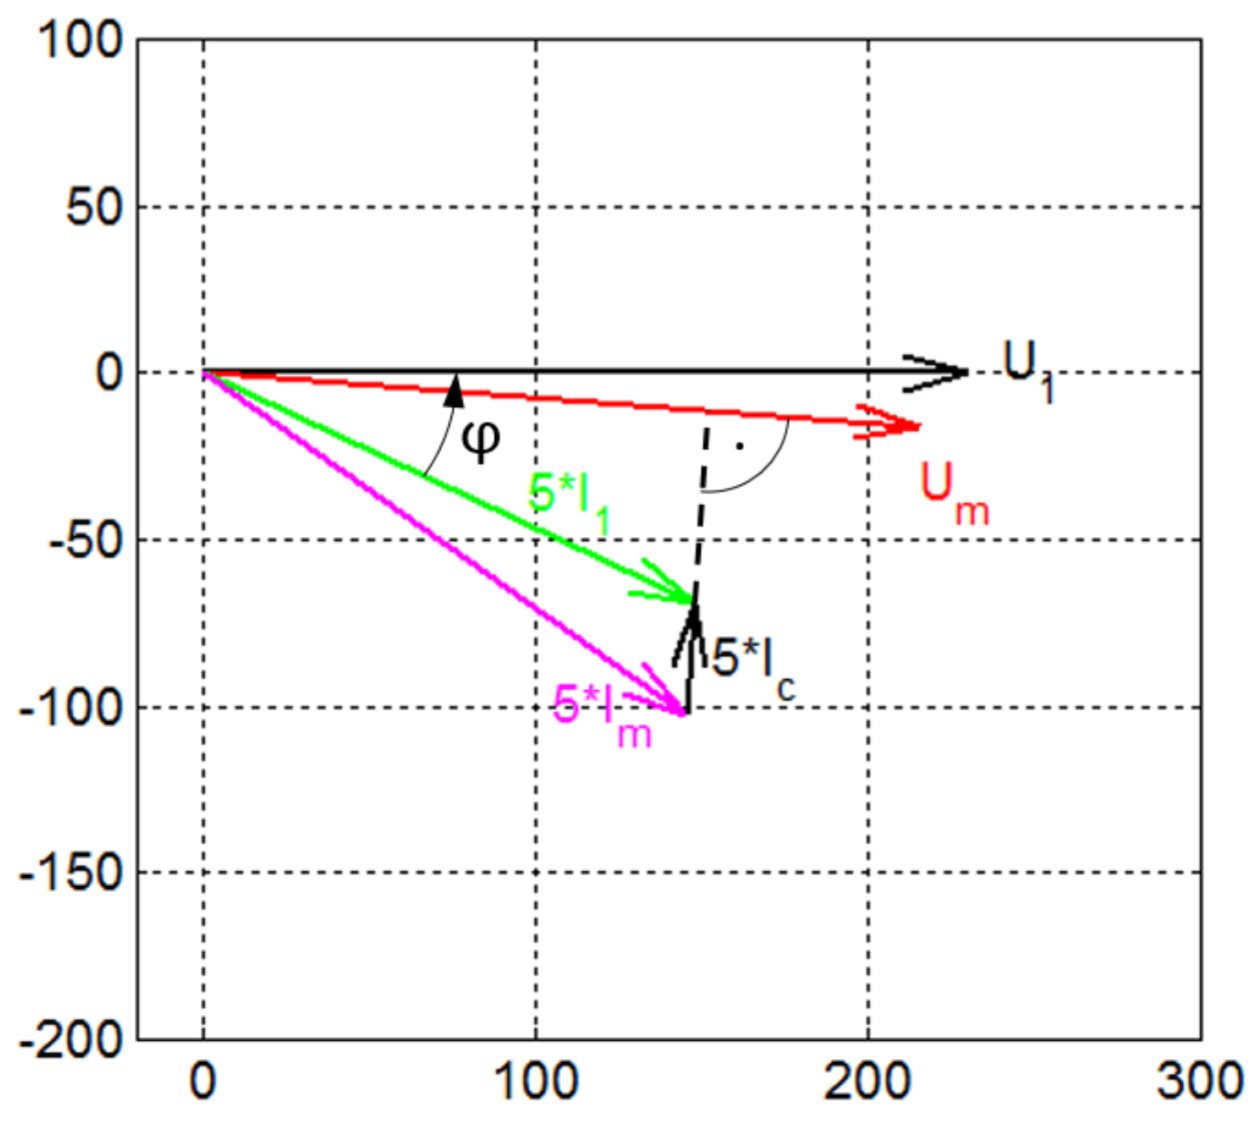
\includegraphics[width=0.9\textwidth]{bilder/a42.png}
\end{minipage}
\begin{minipage}{0.45\textwidth}
Die Ströme aus Aufgabe 1 sind massstabsgetreu einzuzeichnen mit Betrag und Winkel
\end{minipage}

\item Berechnen sie den Kondensator für einen $\cos(\varphi) = 0$\\
Damit der $\cos(\varphi)$ = 1 ist muss der Imaginäranteil der Schaltung = 0 sein. Nicht mit \texttt{pwider(\ldots,\ldots)} arbeiten!

\[
	Z = \left( R_n+R_L + j\omega (L_N+L_L) +\frac{\frac{1}{j\omega C}\cdot (j\omega L_M+R_M)}{\frac{1}{j\omega C}+ (j\omega L_M+R_M)}\right)=0 \quad \texttt{solve(\ldots,C)}
\]

\end{enumerate}
\begin{minipage}[]{0.7\textwidth}
    \begin{circuitikz}
   	  \draw (0,0)
   	  node[rground]{}
   	  to[I, i_=$i(t)$](0,4) node[ocirc]{} node[above]{$E_A$} 
   	  to[R=$R_L$](4,4)
   	  to[L=$L_L$](6,4)
   	  to[short](8,4)
   	  to[R=$R_M$](8,2)
   	  to[L=$L_M$](8,0)
   	  node[rground]{}
   	  ;
      \draw (6,4) node[ocirc]{} node[above]{$E_B$} 
      to[C=$C_K$](6,0)
      node[rground]{}
      ;
    \end{circuitikz}
    
    \end{minipage}
\begin{minipage}[]{0.29\textwidth}
Wobei:\\
- $R_L = 0.2\Omega$\\
- $L_L = 0.1\mu H$\\
- $C_K = 8.3\mu F$\\
- $R_M = 2\Omega$\\
- $L_M = 10mH$\\
- $i(t) = \sqrt{2}\cdot 60A\cdot \sin(2\pi\cdot 50\cdot t)$\\
$+\sqrt{2}\cdot 7A\cdot \sin(2\pi\cdot 250\cdot t)$\\
$+\sqrt{2}\cdot 5A\cdot \sin(2\pi\cdot 550\cdot t)$
\end{minipage}
    \vspace{5mm}
    
    Knotenpotentialmethode:
\[
	\left[\begin{array}{cc}
		\dfrac{1}{R_L+j\omega L_L}&-\dfrac{1}{R_L+j\omega L_L}\\
		-\dfrac{1}{R_L+j\omega L_L}&\dfrac{1}{R_L+j\omega L_L} +\dfrac{1}{R_M+j\omega L_M}+j\omega C_K
	\end{array}\right]
	\cdot \left[\begin{array}{c}
	E_A\\E_B
	\end{array}\right]
	= \left[\begin{array}{c}
	I_{50,250,550}\\0
	\end{array}\right] \vert \omega = 2\pi f
\]
\[
	\left[\begin{array}{cc}
		\dfrac{1}{0.2\Omega+j\omega \cdot 0.1\mu H}&-\dfrac{1}{0.2\Omega+j\omega \cdot 0.1\mu H}\\
		-\dfrac{1}{0.2\Omega+j\omega \cdot 0.1\mu H}&\dfrac{1}{0.2\Omega+j\omega \cdot 0.1\mu H} +\dfrac{1}{2\Omega+j\omega \cdot 10mH}+j\omega 8.3\mu F
	\end{array}\right]
	\cdot \left[\begin{array}{c}
	E_A\\E_B
	\end{array}\right]
	= \left[\begin{array}{c}
	I_{50,250,550}\\0
	\end{array}\right] \vert \omega = 2\pi 50,250,550
\]
\[
	\underbrace{\left[\begin{array}{cc}
	E_A(50Hz)=&328.115V\angle 54.725^\circ\\
	E_B(50Hz)=&318.618V\angle 57.217^\circ
	\end{array}\right]}_{\textrm{ungefährlich da} < \sqrt{2}\cdot 230V}
	\underbrace{\left[\begin{array}{cc}
	E_A(250Hz)=&197.346V\angle 80.298^\circ\\
	E_B(250Hz)=&197.021V\angle 80.866^\circ
	\end{array}\right]}_{\textrm{ungefährlich da} < \sqrt{2}\cdot 230V}
	\underbrace{\left[\begin{array}{cc}
	E_A(550Hz)=&4218.93V\angle 5.403^\circ\\
	E_B(550Hz)=&4217.52V\angle 5.405^\circ
	\end{array}\right]}_{\textrm{Gefährlich da} > \sqrt{2}\cdot 230V}
\]
Optional mit Impedanz und Strömen lösen
\begin{align*}
Z(\omega) &= R_L +j\omega L_L +\frac{1}{j\omega C_M +\frac{1}{R_M+j\omega L_M}} \qquad\vert \omega = 2\cdot \pi \cdot 50, 2\cdot \pi \cdot 250,2\cdot \pi \cdot 550\\
U_M(\omega)&= Z(\omega) \cdot I(\omega)
\end{align*}
\hrule

\begin{minipage}[]{0.7\textwidth}
    \begin{circuitikz}
   	  \draw 
   	  (4.5, 2.5) node[transformer] (T) {}
   	  (0,3)node[ocirc]{} 
   	  to [short,i=$I_1$](1,3)--(3,3) -- (T.A1)
   	  (4, 1.425) node[left] {$N_1$}
      (5, 1.425) node[right] {$N_2$}
      (1.5,3) to [C=$C$](1.5,0)
      (0,3) to [open, v=$U_1$](0,0)
      (T.A2) -- (3,0) -- (0,0)node[ocirc]{}
      (T.B1) -- (6,3) -- (9,3) to [R=$R_L$](9,0) -- (6,0)--(T.B2)
      (7.5,3) to [L=$L_L$](7.5,0)
      (7,3) to [open,v=$U_L$] (7,0)
      ; 
    \end{circuitikz}
\end{minipage}
\begin{minipage}[]{0.29\textwidth}
	\begin{itemize}
	\itemsep0em
	\item $L_L = 0.05H$
	\item $R_L = 15\Omega$
	\item $u(t) = 230V\angle 0^\circ$
	\item $f= 50Hz$
	\item ü $ = \frac{N_1}{N_2} = 8$
	\item $\varphi_k = 0.839$
	\end{itemize}
\end{minipage}


\begin{circuitikz}[american]
\begin{scope}[]
\draw [->] (-1,0) -- (3,0) node[anchor=west] {$P/W$};
\draw [->] (0,-0.5) -- (0,3) node[anchor=west] {$Q/VAr$} ;
\draw [->] (0,0) -- (2.755,0)node[anchor=north] {$P$};
\draw [->] (2.755,0) -- (2.755,2.631)node[anchor=west] {$Q$};
\draw [->] (0,0) -- (2.755,2.631)node[anchor=south east] {$S$};
\draw [->] (2.755,2.631) -- (2.755,1.780)node[anchor=west] {$Q_C$};
\draw [thick,->] (0,0) -- (2.755,1.780)node[anchor=south east] {$S_K$};
%\draw (-1,0) node[anchor=north] {-2} (1,0) node[anchor=south] {2}
%(0,1) node[anchor=west] {4} (0,-1) node[anchor=east] {-4}
%(2,0) node[anchor=north west] {4}
%(-1.5,0) node[anchor=south east] {-3};
%\draw [thick] (-2,-1) -- (-1,1) -- (1,-1) -- (2,0) -- (2.5,.5);
%\draw [dotted] (-1,1) -- (-1,0) (1,-1) -- (1,0)
%(-1,1) -- (0,1) (1,-1) -- (0,-1);
\end{scope}
\end{circuitikz}


\begin{align*}
\underline{Z}_2' &=\underline{Z}_2\cdot \left(\frac{N_1}{N_2}\right)^2  =\frac{1}{\frac{1}{R} +\frac{1}{j\omega L}}\cdot 8^2 =  \frac{1}{\frac{1}{15} +\frac{1}{j 2\pi 50Hz\cdot 0.05H}}\cdot 64 &&= 694.288\Omega\angle 43.679^\circ\\
\underline{I}_1 &= \frac{\underline{U}}{\underline{Z}'_2} = \frac{230V\angle 0^\circ}{694.288\Omega\angle 43.679^\circ} &&=  0.3312A\angle-43.679^\circ\\
\underline{S} &= \underline{U}\cdot \underline{I}_1^*=(230V\angle 0^\circ) \cdot (0.3312A\angle 43.679^\circ)&&= 76.193VA\angle 43.679^\circ\\
P &= \texttt{Real}(S) = \texttt{Real}(76.193VA\angle 43.679^\circ)&&=55.104W\\
Q &= \texttt{Imag}(S) = \texttt{Imag}(76.193VA\angle 43.679^\circ)&&=52.621VAr\\
C &= -\frac{P\cdot (\tan(\arccos(\cos(\varphi_K))-\tan(\varphi))}{\omega \cdot \underline{U}^2} = -\frac{55.104W\cdot (\tan(\arccos(0.839))-\tan(43.679^\circ))}{\omega\cdot (230V\angle 0^\circ)^2}&&=1.016\mu F
\end{align*}

\newpage

\begin{align*}
\underline{U}_{1N} &= 230.94V \angle 0^\circ\\
\underline{U}_{2N} &= 230.94V \angle -120^\circ\\
\underline{U}_{3N} &= 230.94V \angle -240^\circ\\
\underline{Z}_1&= 7\Omega + j\cdot 2\cdot \pi \cdot 50 Hz\cdot 0.3H\\
\underline{Z}_2&= 3\Omega\\
\underline{Z}_3&= 7\Omega\\
\underline{U}_{NN}'&= -\frac{\left( \underline{Y}_1\cdot \underline{U}_{1N} +\underline{Y}_2\cdot \underline{U}_{2N} +\underline{Y}_3 \cdot \underline{U}_{3N} \right)}{\underline{Y}_1+\underline{Y}_2+\underline{Y}_3}\\
 &= -\frac{\frac{1}{(7\Omega + j 2 \pi 50 \cdot 0.3H)}\cdot (230.94V \angle 0^\circ) +\frac{1}{3\Omega}\cdot (230.94V \angle -120^\circ)+\frac{1}{7\Omega} \cdot (230.94V \angle -240^\circ) }{\frac{1}{7\Omega + j\cdot 2\cdot \pi \cdot 50 Hz\cdot 0.3H}+\frac{1}{3\Omega}+ \frac{1}{7\Omega}}\\
&= 142.293V\angle 37.75^\circ\\
U_{1N}' &=U_{1N} + U_{NN}' = (230.94V\angle0^\circ) + (142.293V\angle 37.75^\circ) = (353.412V\angle 14.271^\circ)\\
U_{2N}' &=U_{2N} + U_{NN}' = (230.94V\angle -120^\circ) + (142.293V\angle 37.75^\circ) = (112.093V\angle -91.275^\circ)\\
U_{1N}' &=U_{1N} + U_{NN}' = (230.94V\angle -240^\circ) + (142.293V\angle 37.75^\circ) = (286.317V\angle 90.499^\circ)\\
\end{align*}

\hrule
\vspace{5mm}


\begin{minipage}[]{0.8\textwidth}
\begin{circuitikz}[american inductors]
\draw (0,2) to[sV=$\underline{U}_1$] (0,0)
to[short,i=$I_1$] (2,0)node[ocirc]{}
(2,0) -- (6,0)node[circ]{}
-- (8,0)node[circ]{}
--(14,0)node[ocirc]{}
(0,2) --(2,2)node[ocirc]{}
 	to[R=$R_1$](4,2)
 	to[L=$L_{1\sigma}$](6,2)node[circ]{}
 	to[R=$R_{FE}$](6,0)
(8,2) to[L=$L_{M}$](8,0)
(6,2) --(8,2)node[circ]{} --(8,4)
(8,2)to[L=$L_{2\sigma}'$](10,2)
	to[R=$R_2'$] (12,2)
	to[short,i=$I_2$](13,2)node[ocirc]{}
(8,4)to[L=$L_{3\sigma}'$](10,4)
	to[R=$R_3'$] (12,4)
	to[short,i=$I_3$](14,4)node[ocirc]{}
(13,2)to[open,v^=$\underline{U}_2'$](13,0)
(14,4)to[open,v^=$\underline{U}_3'$](14,0) 
;
\end{circuitikz}


\end{minipage}
\begin{minipage}{0.19\textwidth}
Nennbetrieb:
\begin{itemize}
\itemsep0em
\item $U_1 = 230V$
\item $f= 50$Hz
\item $U_2 = $ 24V
\item $U_3 = $ 12V
\item $P_1 = P_2+P_3+P_{FE} +P_{CU}$
\item $P_2 = 1.7kW$
\item $P_3 = 1.3kW$
\end{itemize}
\end{minipage}

\vspace{5mm}
\begin{minipage}{0.49\textwidth}
Leerlauftest:
\begin{itemize}
\itemsep0em
\item $S_0 = P_{FE} + j\cdot Q_\mu$
\item  $\qquad = 75W +j\cdot 95 VAr$
\end{itemize}
\end{minipage}
\begin{minipage}{0.49\textwidth}
Kurzchluss an $U_2, U_3$
\begin{itemize}
\item $S_K = P_{cu}+j\cdot Q_\sigma$
\item $ \qquad= 110W+ j\cdot 120 VAr$
\end{itemize}
\end{minipage}

\begin{align*}
R_{FE} &= \frac{U_1^2}{P_{FE}} = \frac{(230V)^2}{75W} = 705.333\Omega\\
L_M &= \frac{U_1^2}{Q_\mu\cdot \omega} = \frac{(230V)^2}{95VAr\cdot 2\pi\cdot 50Hz} = 1.77H\\
I_{2K} &=  \frac{P_2}{U_{2N}} = \frac{1700W}{24V} = 70.833A\\
I_{1K} &= \frac{P_3}{U_{3n}} = \frac{1300W}{12V} = 108.333A\\
Z_K^*&= \frac{U_0^2}{S_K} = \frac{(230V)^2}{(110W+ j\cdot 120 VAr)} = (219.355 -j\cdot 239.547)\Omega\\
R_1 &= R'_2\vert \vert R'_3\quad\Rightarrow = \frac{\texttt{Real}(Z_K)}{2} = 109.79\Omega\\
X_{\sigma 1}&= X'_{\sigma 2} \vert \vert X'_{\sigma 3}\quad \Rightarrow = \frac{\texttt{Imag}(Z_K)}{2} = 119.774\Omega\\
\end{align*}

\newpage




